\documentclass [nobachelor,english,a4paper,11pt,oneside,webreferences,glossary,indextop,listoflistings,nolistofalgorithms]{INSOthesis}
% change encoding in the document
%\inputencoding{utf8} % default
%\inputencoding{latin1} % for windows

\thesistitle{An Agent Based Simulation of Geospatial Aspects of Street Crime in Maputo City}
\thesisshorttitle{Simulation of Geospatial Aspects of Street Crime}
%\thesissubtitle{Optional Subtitle} % optional
\thesisdate{\today}

% all titles and designations have to be gender-related!
\thesistype{Diplomarbeit}{Master's Thesis}
\thesisdegree{Diplom-Ingenieur}{Master of Engineering}
\thesiscurriculum{Business Informatics}{Business Informatics} % your study
\thesisauthor{Philipp Schnatter} % your name
\thesisauthoraddress{Puchsbaumgasse 62/10, 1100 Wien} % your address
\thesismatrikelno{0325962} % your registration number

% advisor
%\thesisauthorpreamble {Verfasser}
%\thesisadvisorpreamble {Betreuung}
\thesisadvisorone {Thomas Grechenig}
\thesisadvisortwo {Paul Pöltner}
%\thesisadvisorthree {Vorname Nachname}

% Bibliographie file
\bibliography{bibliography/references}

\hypersetup{
  %colorlinks=false % enable and disable frames arround links
}

%%%%%%%%%%%%%%%%%%%%%%%%%%%%%%%%%%%%%%%%%%%%%
%
% Can be used to add additional informations
%
%%%%%%%%%%%%%%%%%%%%%%%%%%%%%%%%%%%%%%%%%%%%%
% \AfterTitlePages{}
% \AfterDeclaration{}
% \AfterAcknowledgements{}
% \AfterAbstract{}
% \AfterListOfFigures{}
% \AfterListOfTables{}
% \AfterAbbreviations{}
% \AfterBibliography{}

\renewcommand\afterchapternum{\hspace{1em}}
\begin{document}

\maketitle

%%%%%%%%%%%%%%%%%%%%%%%%%%%%%%%%%%%%%%%%%
%%%   CONTENTS    %%%%%%%%%%%%%%%%%%%%%%%
%%%%%%%%%%%%%%%%%%%%%%%%%%%%%%%%%%%%%%%%%

%%%%%%%%%%%%%%%%%%%%%%%%%%%%%%%%%%%%%%%%%%%%%%%%%%%%%%%%%%%%%%%%%%%%%%%%
\chapter{Einleitung}
\label{sec:introduction}
%%%%%%%%%%%%%%%%%%%%%%%%%%%%%%%%%%%%%%%%%%%%%%%%%%%%%%%%%%%%%%%%%%%%%%%%

\makeatletter
\ifthesis@masterthesis
Das hier zur Verfügung gestellte Template ist als Hilfestellung gedacht, sie stellt keine verbindliche Richtlinie dar. Der Aufbau einer Diplomarbeit hängt sehr von der bearbeiteten Thematik ab. Diese Vorlage ist für eine Arbeit erstellt, die einen experimentellen Teil enthält (Fallbeispiel). Bei theoretischen Arbeiten oder Programmierungen sind entsprechende Anpassungen vorzunehmen, bitte Rücksprache mit Ihrem Betreuer halten. Bei der Gliederung der Arbeit ist darauf zu achten, dass das Inhaltsverzeichnis einen ersten Eindruck von der thematischen Vollständigkeit sowie der Ausgewogenheit der Behandlung des Themas bietet. Die Gliederung und somit auch der Wahl der Kapitelüberschriften vermitteln einen Eindruck über die angewendete Systematik, die Vollständigkeit der Behandlung des Themas und deren \enquote{Wissenschaftlichkeit}.
\fi
\makeatother

In der Einleitung soll die Zielsetzung der Arbeit beschrieben, ihre Einordnung in einen übergeordneten Kontext hergestellt und die Bedeutung des Themas erörtert werden. Zu diesem Zweck ist die Einleitung in folgende Unterkapitel unterteilt:
\begin{itemize}
	\item Problemstellung
	\item Motivation
	\item Zielsetzung
	\item Aufbau der Arbeit
\end{itemize}

\makeatletter
\ifthesis@masterthesis
Durch die Einleitung sollen folgende Punkte in den jeweiligen Unterkapiteln klargestellt werden:
\begin{itemize}
	\item Etwaige thematische Einschränkungen bzw. Auswahl und Begründung der Bearbeitungsziele
	\item Betrachtung verschiedener methodischer Alternativen zur Aufgabenlösung und Erklärung der Entscheidung
	\item Gewählter Lösungsansatz, z.B. theoretische Untersuchung, Literaturauswertung und -vergleich oder eine empirische, auf eigenen Erhebungen basierende Untersuchung
\end{itemize}
\fi
\makeatother

\paragraph{Organisatorisches}
\makeatletter\ifthesis@masterthesis
Bitte einen Zeitplan für die Verfassung Ihrer Diplomarbeit erarbeiten und mit Ihrem Betreuer abstimmen. Es gibt sehr \enquote{kurzlebige} Themenstellungen, die rasch an Aktualität verlieren, da ist der Zeitplan unbedingt einzuhalten, ansonsten wird das Thema neu vergeben. Bei Themen, die länger aktuell bleiben, kann der Zeitrahmen auch länger erstreckt werden, dies aber bitte im Vorfeld abklären! Üblicherweise sollte die Verfassung einer Diplomarbeit ein halbes Jahr bis ein Jahr dauern, Ausnahmen bitte zumindest durch regelmäßigen email-Kontakt abstimmen.
\fi\makeatother

Der Umfang einer Diplomarbeit beträgt üblicherweise 90 bis ca. 120 Seiten und bei Bachelorarbeiten 40 bis ca. 60 Seiten. Beurteilungskriterien für eine Diplomarbeit ist nicht nur die Qualität der praktischen Arbeit, sondern auch Aufbau, Inhalt und Formulierung der schriftlichen Arbeit. Insbesondere sind die Grundregeln wissenschaftlichen Arbeitens (z.B. richtiges Zitieren) zu beachten.

\paragraph{Allgemeines}
Achtung beim Setzen von Absätze.

Fußzeilen: Bei technischen Arbeiten eher unüblich. \\
In den Sozialwissenschaften (z.B. BWL) ist es üblich, die Referenz in eine Fußnote zu setzen.
\\
In den technischen Wissenschaften ist es üblich, im Text ein Kürzel (Dorn et al. 1999) oder eine Zahl [1] zu verwenden, um dann im Anhang der Arbeit alle Referenzen detailliert aufzuführen, wobei jede Referenz mit dem Kürzel beginnt.

Bei einer wissenschaftlichen Arbeit wird Wert auf die Einhaltung formaler Aspekte des guten Schreibens gelegt. Es ist hilfreich, wenn man seinen eigenen Schreibstil kritisch in Bezug auf folgende Punkte überprüft:
\begin{itemize}
	\item Einfachheit (das \ac{KISS}-Prinzip gilt nicht nur für die Softwareentwicklung, sondern auch für wissenschaftliche Arbeiten: Mach es schlicht und wesentlich/\acl{KISS})
	\item Gliederung/ logische Ordnung (vom Allgemeinen zum Konkreten, nachvollziehbare Kette von einer Fragestellung/ einem Problem über die Bearbeitung und Zerlegung in Detailprobleme zur Lösung und der Ableitung von Erkenntnissen)
	\item Kürze/Prägnanz (keine Schachtelsätz, Wiederholungen vermeiden – \enquote{Don't repeat yourself})
	\item Anregende Zusätze (erläuternde/ interessante/ spannende Praxisbeispiele etc.)
	\item Sprache/Stil (kein Erzählstil, möglichst keine \enquote{ich}-Form, objektiv)
	\item Korrekte Formeln und Abbildungen
	\item Korrekte Zitierweise (siehe Kapitel Literaturverzeichnis)
	\item Einhaltung definierter Rahmenbedingungen (z.B. diese Vorlage)
	\item Vermeiden von Anglizismen. Grundsätzlich sollte in einer in Deutsch verfassten Diplomarbeit immer das deutsche Wort verwendet werden, wenn es unmissverständlich und akzeptiert ist. Ein Eindeutschen um jeden Preis ist allerdings zu vermeiden, da dies zu schwer lesbaren Texten führt. Beispiele: Der Begriff \enquote{Unterbrechung des Programmflusses} ist angebrachter als \enquote{Interrupt des Programmflusses}, und \enquote{verdeckte Kanäle} ist als akzeptierter deutscher Begriff für \enquote{Covert Channels} zu verwenden. Umgekehrt ist aber \enquote{Cursor} das bessere Wort als \enquote{Lichtmarke}. Anglizismen können als Stilmittel genutzt werden, etwa wenn man von einer \enquote{Quick and Dirty} Implementierung spricht.
\end{itemize}

\paragraph{Typographie}
Grundsätzlich sollten nicht mehr als drei unterschiedliche Schriftarten verwendet werden. Grundsätzlich sollte die Typographie sowie die Anordnung von Bildern, Tabellen, etc. \LaTeX überlassen werden. Allerdings können Silbentrennungen durch \verb|\-| gesteuert werden.

Abweichungen nach persönlichem Geschmack und in Rücksprache mit Ihrem Betreuer sind zulässig. Als Stilmittel werden üblicherweise nur die Fettschrift und Kursivschrift verwendet - Unterstreichungen, Schattenschriften etc. sind zu vermeiden. Blocksatz bitte mit automatischer Silbentrennung verwenden, Rechtschreibprüfung aktivieren.

Generell kann bei der Einleitung eine modifizierte Version des Exposés als Basis verwendet werden.

%=======================================================================
\section{Problemstellung}
%=======================================================================

Formulierung der Problemstellung, Einbettung in das Forschungsumfeld und Theorie, auf die sich die Arbeit beziehen. Tendenziell kurz, allgemeiner und sehr gut verständlich -- detaillierter im Kapitel \enquote{Grundlagen}.

Die formulierte Fragestellung soll das Interesse an der Lösung wecken (eine langweilige oder triviale Problemstellung lässt meistens auch eine eher weniger interessante wissenschaftliche Arbeit erwarten).

\makeatletter\ifthesis@masterthesis
Nach dem Lesen dieses Kapitels sollten folgende Punkte klar dargestellt sein:
\begin{itemize}
	\item Welche konkrete Fragestellung/Arbeitshypothese/welches Problem liegt dem Thema zugrunde?
	\item Klare Definition des Untersuchungsgegenstands (z.B. effiziente Internationalisierung/ Mehrsprachigkeit von Computerprogrammen im Java Umfeld).
	\item Darlegung und Begründung thematischer Abgrenzungen.
	\item Klare Darstellung eines ggf. übergeordneten fachlichen Kontexts/Zusammenhangs (z.B. des medizinisch/ organisatorischen Rahmens, der bei einer Arbeit über Usability einen Einfluss auf die Usability einer auf Tablets/Touchscreens basieren Pflegedokumentation im klinischen Bereich hat).
\end{itemize}

In diesem Kapitel wird das Problem und sein Kontext beschrieben (\enquote{die Sache/die Frage}) – nicht aber, warum es gerade zum Zeitpunkt der Diplomarbeit notwendig ist, für dieses Problem eine Lösung zu erarbeiten. Das \enquote{Warum} (die Motivation) wird im nächsten Unterkapitel beschrieben.
\fi\makeatother

%=======================================================================
\section{Motivation}
%=======================================================================

In diesem Kapitel wird der Forschungsbedarf aufgezeigt. Nach dem Lesen dieses Kapitels sollten folgende Punkte klar dargestellt sein:
\begin{itemize}
	\item Aktueller Stand der Wissenschaft in Bezug auf die zuvor formulierte Problemstellung und klare Darstellung, was hier unzureichend/offen ist.
	\item GGf. Darstellung des größeren Forschungsbereichs, in den die Diplomarbeit eingebettet ist.
	\item Darlegung der Bedeutung des Themas für den Stand oder die Weiterentwicklung eines Bereichs der Informatik (z.B. Datenbanksysteme, Mobile Anwendungen, Java-Programmierung, Rechenzentrumsbetrieb, \dots) oder eines Fachbereichs (z.B. Bankwesen, Wertpapierhandel, Gesundheitswesen, Transportwesen, Flugsicherheit \dots). Erklärung, was durch die Lösung des Problems z.B. kostengünstiger/schneller/hochwertiger/sicherer/anwendbarer/\enquote{schöner} etc. wird.
\end{itemize}

%=======================================================================
\section{Zielsetzung}
%=======================================================================

Nachdem die Problemstellung und die Motivation zu deren Lösung formuliert wurden, wird in diesem Kapitel das zu erarbeitende Resultat beschrieben.

\makeatletter\ifthesis@masterthesis
Nach dem Lesen dieses Kapitels sollten folgende Punkte klar dargestellt sein:
\begin{itemize}
	\item Umfang, in dem die Problemstellung am Ende der Arbeit gelöst sein soll bzw. mit welchen Einschränkungen.
	\item Methode zur Erarbeitung des Resultats.
	\item Gibt es einen Theorie- und einen Praxisteil?
	\item Schwerpunkte des Praxisteils (z.B. Durchführung einer Umfrage, Programmierung, Herstellung von Hardware, Erprobung einer Methode in einem konkreten Projekt)?
	\item Art des Resultats (z.B. ein Programm, eine Formel, eine Methode, die Erweiterung einer existierenden Methode, ein Konzept, ein Framework, Hardware-Prototyp, eine bewiesene Erkenntnis)?
\end{itemize}
\fi\makeatother

\makeatletter\ifthesis@masterthesis
%=======================================================================
\section{Aufbau der Arbeit}
%=======================================================================

Beispielhaft:

Kapitel \ref{sec:fundamentals} behandelt sowohl Grundlagen als auch Definitionen und bietet einen Überblick \dots, die als Basis für \dots dienen.

\dots, wird in Kapitel 3 erläutert..

Ein Anwendungsszenario (Fallbeispiel), das \dots, ist in Kapitel 4 dargestellt. Dieses Szenario umfasst \dots.

Kapitel 5 setzt sich \dots. auseinander.

Einsatzmöglichkeiten in der Praxis werden in Kapitel 6 diskutiert.

Abschließend fasst Kapitel \ref{sec:conclusion} die wesentlichen Erkenntnisse zusammen und gibt einen Ausblick in die Zukunft.
\fi\makeatother

%%%%%%%%%%%%%%%%%%%%%%%%%%%%%%%%%%%%%%%%%%%%%%%%%%%%%%%%%%%%%%%%%%%%%%%%%%%%%%%%%%%%%%%%%%%%%%%%%%%%%%%%%%%%%%%%%%%%%%%%%%%%%%%%%%%%%%%%%%%%%%%%%%%%%%%%%%%%%%%%%%%%%%%%%%
% \section{General Information}
%
% This document is intended as a template and guideline and should support the author in the course of doing the master's thesis.
% Assessment criteria comprise the quality of the theoretical and/or practical work as well as structure, content and wording of the written master's thesis. Careful attention should be given to the basics of scientific work (e.g., correct citation).\footnote{Sample Footnote}
%
% \section{Organizational Issues}
%
% A master's thesis at the Faculty of Informatics has to be finished within six months. During this period regular meetings between the advisor(s) and the author have to take place.
% In addition, the following milestones have to be fulfilled:
% \begin{enumerate}
%   \item  Within one month after having fixed the topic of the thesis the master's thesis proposal has to be prepared and must be accepted by the advisor(s). The master's thesis proposal must follow the respective template of the dean of academic affairs. Thereafter the proposal has to be applied for at the deanery. The necessary forms may be found on the web site of the Faculty of Informatics. \url{http://www.informatik.tuwien.ac.at/dekanat/formulare.html}
%   \item  Accompanied with the master's thesis proposal, the structure of the thesis in terms of a table of contents has to be provided.
%   \item Then, the first talk has to be given at the so-called ``Seminar for Master Students''. The slides have to be discussed with the advisor(s) one week in advance. Attendance of the ``Seminar for Master Students'' is compulsory and offers the opportunity to discuss arising problems among other master students.
%   \item At the latest five months after the beginning, a provisional final version of the thesis has to be handed over to the advisor(s).
%   \item As soon as the provisional final version exists, a first poster draft has to be made. The making of a poster is a compulsory part of the ``Seminar for Master Students'' for all master studies at the Faculty of Informatics. Drafts and design guidelines can be found at \url{http://www.informatik.tuwien.ac.at/studium/richtlinien}.
%   \item After having consulted the advisor(s) the second talk has to be held at the ``Seminar for Master Students''.
%   \item At the latest six months after the beginning, the corrected version of the master's thesis and the poster have to be handed over to the advisor(s).
%   \item After completion the master's thesis has to be presented at the ``epilog''. For detailed information on the epilog see: \\ \url{http://www.informatik.tuwien.ac.at/studium/epilog}
% \end{enumerate}
%
% \section{Structure of the Master's Thesis}
%
% If the curriculum regulates the language of the master's thesis to be English (like for ``Business Informatics''), the thesis has to be written in English. Otherwise, the master's thesis may be written in English or in German. The structure of the thesis is predetermined.
% The table of contents is followed by the introduction and the main part, which can vary according to the content. The master's thesis ends with the bibliography (compulsory) and the appendix (optional).
%
% \begin{itemize}
%   \item	Cover page
%   \item Acknowledgements
%   \item Abstract of the thesis in English and German
%   \item Table of contents
%   \item Introduction
%   	\begin{itemize}
%   		\item motivation
%   		\item problem statement (which problem should be solved?)
%   		\item aim of the work
%   		\item methodological approach
%   		\item structure of the work
%   	\end{itemize}
%   \item State of the art / analysis of existing approaches
%   	\begin{itemize}
%   		\item literature studies
%   		\item analysis
%   		\item comparison and summary of existing approaches
%   	\end{itemize}
%   \item Methodology
%   	\begin{itemize}
%   		\item used concepts
%   		\item methods and/or models
%   		\item languages
%   		\item design methods
%   		\item data models
%   		\item analysis methods
%   		\item formalisms
%   	\end{itemize}
%   \item Suggested solution/implementation
%   \item Critical reflection
%   	\begin{itemize}
%   		\item comparison with related work
%   		\item discussion of open issues
%   	\end{itemize}
%   \item Summary and future work
%   \item Appendix: source code, data models, \dots
%   \item Bibliography
% \end{itemize}
%

%%%%%%%%%%%%%%%%%%%%%%%%%%%%%%%%%%%%%%%%%%%%%%%%%%%%%%%%%%%%%%%%%%%%%%%%
\chapter{Grundlagen}
\label{sec:fundamentals}
%%%%%%%%%%%%%%%%%%%%%%%%%%%%%%%%%%%%%%%%%%%%%%%%%%%%%%%%%%%%%%%%%%%%%%%%

In diesem Kapitel werden die theoretischen Grundlagen und alle in der Arbeit verwendeten und für das Verständnis relevante Begriffe erläutert. Kapitelnamen spezifizieren, anpassen an die Fragestellung der Arbeit.

\makeatletter\ifthesis@masterthesis
Nach dem Lesen dieses Kapitels sollten folgende Punkte klar dargestellt sein:
\begin{itemize}
	\item Beschreibung der relevanten theoretischen Grundlagen für die Behandlung der Fragestellung
	\item Detaillierte Beschreibung ggf. vorhandener relevanter Spezifika des Anwendungsbereichs, in dem das Problem gelöst wird
	\item Detaillierte Beschreibung relevanter Spezifika eingesetzter Technologien
	\item Analyse bestehender Ansätze/ Vorarbeiten: Literaturstudium, Analyse, Vergleich und Zusammenfassung bestehender Ansätze.
\end{itemize}
\fi\makeatother

Gerade im Bereich der Grundlagen wird viel Literatur zitiert -- Details zum Zitieren finden Sie im Kapitel \ref{sec:references}. Da keine Diplomarbeit so innovativ ist, dass sie nicht auf vorhandenes Wissen aufbaut und in ein entsprechendes Forschungsumfeld eingebettet ist, kommt an dieser Stelle der Literaturrecherche eine besondere Bedeutung zu. Als Daumenregel gilt, dass der aktuelle Stand der Wissenschaft in der Informatik üblicherweise durch Publikationen v.a. der letzten 2 – 4 Jahre repräsentiert wird.

\makeatletter\ifthesis@masterthesis
Beispielhaft einleitender Text an dieser Stelle:\\
Dieses Kapitel stellt Konzepte der Informationstheorie vor und liefert theoretische Grundlagen zu verdeckten Kanälen. Die verdeckte Kommunikation wird mit den verwandten Techniken der Steganographie und Kryptographie verglichen. Außerdem werden ein einfaches Fehlerkorrekturverfahren sowie die Grundlagen des HTTP-Protokolls beschrieben.
\fi\makeatother

%=======================================================================
\section{Aktueller Stand der Technik}
%=======================================================================

In diesem Kapitel wird ein Überblick über bereits existierende Lösungen für die Problemstellung bzw. verwandte Problemstellungen gegeben. Dabei ist eine Klassifizierung der existierenden Lösungen empfehlenswert. Eine Analyse der Lösungen, nach Kriterien sortiert, sollte insbesondere auch die Defizite der existierenden Lösungen erläutern und damit insbesondere auch eine Begründung liefern, warum diese Lösungen für die Problemstellung der Arbeit nicht herangezogen werden können.

%-----------------------------------------------------------------------
\subsection{Unterkapitel}
%-----------------------------------------------------------------------

Bei der Verwendung von Gliederungsebenen gibt es Folgendes zu beachten:
\begin{itemize}
	\item Es sollten nicht mehr als 3 Gliederungstiefen nummeriert werden.
	\item Unterkapitel sind nur dann sinnvoll, wenn es auch mehrere Untergliederungen gibt. Ein Kapitel 2.1.1 sollte somit nur dann verwendet werden, wenn es auch 2.1.2 gibt.
	\item Oft ist es einfacher und besser verständlich, Aufzählungen als Text zu formulieren und somit weitere Gliederungsstufen zu vermeiden.
\end{itemize}

%-----------------------------------------------------------------------
\subsection{Abbildungen}
\label{sec:abbildungen}
%-----------------------------------------------------------------------

Beschreibungen zu Abbildungen und Tabellen stehen unter dem Bild. Jede Abbildung muss im Fließtext referenziert werden. In \LaTeX besitzen Abbildungen typischerweise Labels, welche zum referenzieren verwendet werden. Zudem plaziert \LaTeX die Abbildungen an geeigneten Stellen, was meistens auch wünschenswert ist. Falls das nicht gewünscht wird, kann es durch Optionen beeinflusst werden.

Abbildung \ref{fig:xxx} verdeutlicht  \dots\\
(siehe Abbildung \verb|\ref{<label>}|)

\begin{figure}
	\centering
	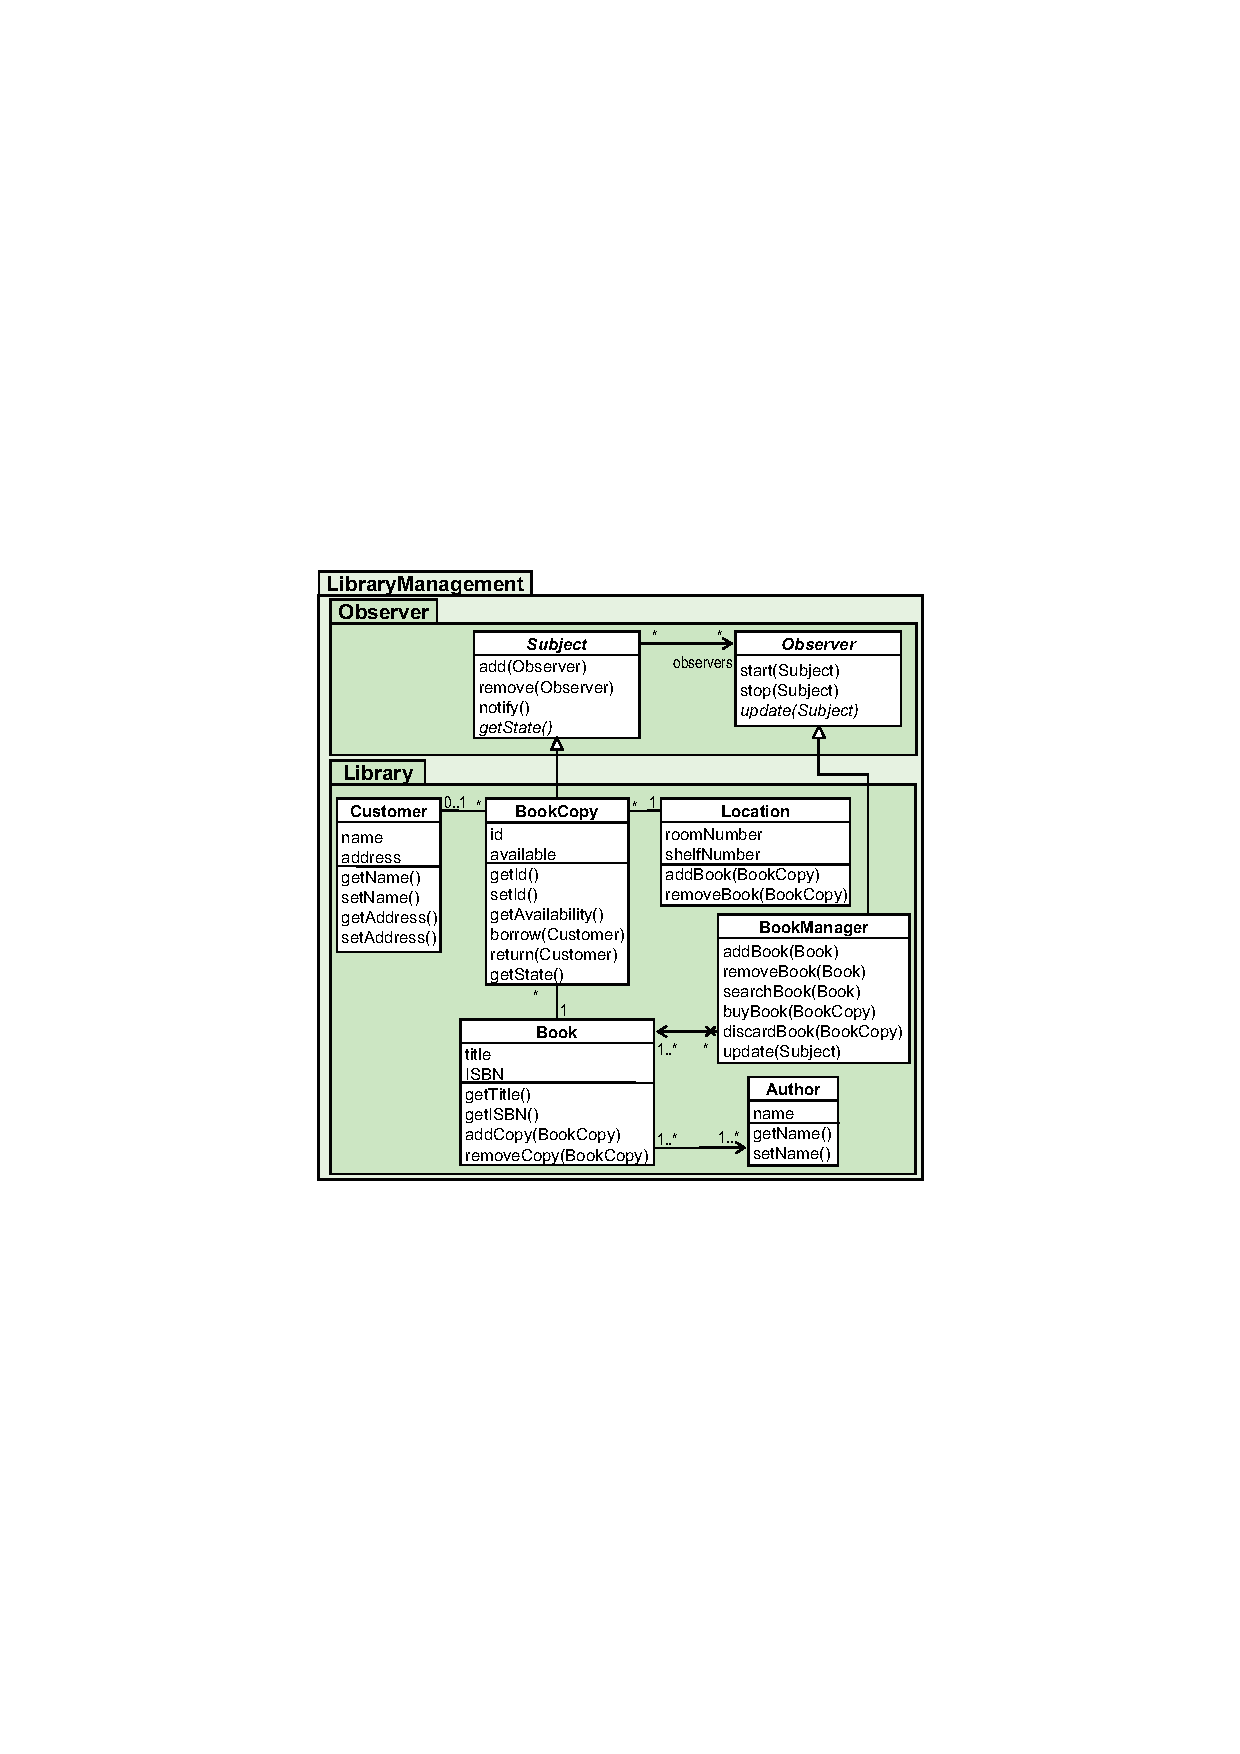
\includegraphics[width=0.4\linewidth]{figures/figure1}
	\caption{xxx (Quelle zitieren, wenn nicht selbst erstellt)}
	\label{fig:xxx}
\end{figure}

%-----------------------------------------------------------------------
\subsection{Tabellen}
%-----------------------------------------------------------------------

Jede Tabelle muss im Fließtext referenziertw werden. Für Tabellen gelten die selben Regeln, wie für Abbildungen (siehe dazu Abschnitt \ref{sec:abbildungen}).

Eine Beispiel einer Tabelle ist in Tabelle \ref{tab:xxx} zu finden:
\begin{table}
	\centering
	\begin{tabular}{| >{\bfseries}l | c | r | }
		\hline
			\rowcolor{orange} \bfseries Linksbündig & \bfseries Zentriert & \bfseries Rechtsbündig \\
		\hline
		\hline
			Zeile 1 & xxx & xxx \\\hline
			Zeile 2 & xxx & \dots \\\hline
			\multirow{2}{*}{Zeile3}
			& xxx & xxx \\\cline{2-3}
			& xxx & xxx \\\hline
		\hline
			\multicolumn{3}{| c |}{xxx} \\\hline
	\end{tabular}
	\caption{xxx (Quelle angeben)}
	\label{tab:xxx}
\end{table}

Bitte beachten Sie, dass Tabellen generell so einfach wie möglich gehalten werden sollen. Tabelle \ref{tab:xxx} dient unter anderem dazu Studierenden zu zeigen, wie Tabellen in \LaTeX\xspace erstellt werden können und wie Farben verwendet werden.
%%%%%%%%%%%%%%%%%%%%%%%%%%%%%%%%%%%%%%%%%%%%%%%%%%%%%%%%%%%%%%%%%%%%%%%%
\chapter{Konkrete Problemstellung -- Umfeldbeschreibung}
\label{sec:problemdescription}
%%%%%%%%%%%%%%%%%%%%%%%%%%%%%%%%%%%%%%%%%%%%%%%%%%%%%%%%%%%%%%%%%%%%%%%%

In diesem Kapitel wird die eigentliche Problemlösung in einem oder mehreren Unterkapiteln ausgeführt. Die Strukturierung dieser Kapitel ist naturgemäß sehr stark von der konkreten Aufgabenstellung abhängig. Der Name dieses Kapitels ist anzupassen, z.B. Umfeldbeschreibung -- Fallbeispiel \dots, konkreter schreiben je nach Art Diplomarbeit/Fragestellung.
\makeatletter\ifthesis@masterthesis
Nachfolgend einige Beispiele für unterschiedliche Arten von Diplomarbeiten.

Bei einer Software-Entwicklungsarbeit bieten sich folgende Unterkapitel an:
\begin{itemize}
	\item Im Kapitel \enquote{Design} sollte die konzeptionelle Lösung vorgestellt, diskutiert und begründet werden. Das Ergebnis dieses Kapitels könnte beispielsweise eine Protokoll-Architektur sein.
	\item Im Kapitel \enquote{Modelle} erfolgt üblicherweise das Feindesign. In diesem Kapitel könnten beispielsweise einzelne Protokolle bzw. Algorithmen aus der vorher definierten Protokoll-Architektur eingeführt und diskutiert werden. Achtung: Generell darauf achten, bei der eingangs erläuterten Notation zu bleiben und nicht Synonyme zu verwenden, verwirrt den Leser.
	\item Das Kapitel \enquote{Implementierung} sollte sich dann vorwiegend mit den Details der Umsetzung befassen. In diesem Kapitel sollte nur im Ausnahmefall exemplarisch Quellcode vorgesehen werden. Vielmehr sollten alle Probleme, die bei der Realisierung aufgetreten sind, dokumentiert, interpretiert und die Lösung erläutert werden.
\end{itemize}

Bei einer Arbeit zu einem abstrakteren Thema, bei dem ein oder mehrere Fallbeispiele aus der industriellen Praxis bearbeitet werden, bieten sich folgende Unterkapitel an:
\begin{itemize}
	\item Im Unterkapitel \enquote{Analyse der Problemstellung} wird die konkrete Problemstellung (die Situation im betrachteten Unternehmen) der Fallbeispiele beschrieben. Das Ergebnis dieses Kapitels könnte eine schematische Netzwerk- oder Applikationsarchitektur sein.
	\item Im Unterkapitel \enquote{Fallbeispiel} sollte sich (analog zur Implementierung in der Software-Entwicklung) mit den konkreten Details der Umsetzung befassen. Hier wird dargelegt, wie das zuvor identifizierte Lösungsschema konkret zur Anwendung gelangen kann bzw. welche Probleme während des Umsetzungsprojekts aufgetreten sind.
\end{itemize}

Bei einer Arbeit, deren Grundlage eine Auswahl eines Softwaresystems ist, bieten sich folgende Unterkapitel an:
\begin{itemize}
	\item IST-Analyse
	\item Hardware und Softwareausstattung
	\item Beschreibung der Geschäftsprozesse
	\item Schwachstellenanalyse des Unternehmens
	\item SOLL-Konzeption
	\item Auswahlverfahren möglicher verfügbarer Systeme -- Kriterienkatalog
	\item Einführung des neuen Systems
\end{itemize}

Bei einer Arbeit, deren Fokus auf der Durchführung und Auswertung von Fragebögen liegt, bieten sich folgende Unterkapitel an:
\begin{itemize}
	\item Im Kapitel \enquote{Problemstellung und Fragebogendesign} wird die fachliche Problemstellung detailliert erläutert und der Inhalt des Fragebogens in Bezug zur Problemstellung dargestellt.
	\item Im Kapitel \enquote{Befragungsmethode} werden die Untersuchungsobjekte (z.B. Praktische Ärzte), die Grundgesamtheit (Anzahl praktische Ärzte in Venezuela), Stichprobengesamtheit und das Verfahren zur Stichprobenziehung und das Erhebungsverfahren (Verteilung und Rücklauf der Fragebögen) beschrieben.
	\item Im Kapitel \enquote{Auswertungsmethode} werden die möglichen Auswertungsmethoden aufgelistet und ggf. begründet die ausgewählte Methode beschrieben.
	\item Im Kapitel \enquote{Befragungsdurchführung} wird die Untersuchungsdurchführung (z.B. Zeit, Ort der Befragung, Zeitraum der gesamten Befragung, besondere für das Untersuchungsergebnis oder zukünftige Forschungsarbeiten relevante Vorkommnisse etc.) dargestellt.
\end{itemize}

Hier intensive Rücksprache mit Ihren jeweiligen Fachbetreuern halten, mehrere Diplomarbeiten der Fakultät zu diesem Themenbereich durchsehen. Unabhängig vom Typ der Diplomarbeit werden im nachfolgenden Kapitel die konkreten Ergebnisse beschrieben.
\fi\makeatother
\chapter{Hinweise zur Literatur}
\label{sec:references}

\section{Literatursuche}

Der Vollzugang zu einigen Publikationen ist nur intern aus dem TU-Netz möglich. Um auf möglichst viele Papers extern zugreifen zu können, wird von der TU Wien eine \href{http://www.zid.tuwien.ac.at/tunet/vpn/extern/}{VPN-Zugangsmöglichkeit} angeboten, diesen VPN-Zugang bitte gleich einrichten.

Besonders ergiebig sind folgende Search-Engines:\\
\href{http://academic.research.microsoft.com/}{Microsoft Academic}\\
\href{http://dl.acm.org/}{ACM-Datenbank}\\
\href{http://scholar.google.com/}{Google Scholar}

Wir empfehlen, vor Beginn Ihrer Arbeit einige Diplomarbeiten, die am INSO oder generell an der Fakultät für Informatik verfaßt wurden, zu Ihrem Themenbereich zu suchen und Aufbau, Schreibstil, Art der Abbildungen etc. durchzuschauen. Arbeiten finden Sie \href{http://media.obvsg.at/tuw?query=grechenig&metaname=swishdefault&submit=Suche+starten&sbm=tuw*&lbm=*&lbc=*&searchtype=sim&.cgifields=metaname}{hier}.

Weitere Datenbanken und Suchmaschinen:\\
\href{http://rzblx1.uni-regensburg.de/ezeit/search.phtml?bibid=UBTUW&colors=7&lang=de}{Elektronische Zeitschriftenbibliothek der TU Wien}\\
\href{http://citeseer.ist.psu.edu/index;jsessionid=BF9BD5A89D42210F60E5CA88B40BAD9C}{Scientific Literature Digital Library (CiteSeer)}\\
\href{http://www.ingentaconnect.com/}{Ingenta}\\
\href{http://www.theiet.org/resources/inspec/}{INSPEC}

Journals:\\
\href{http://ieeexplore.ieee.org/}{IEEE - Institute of Electrical and Electronics Engineers, Inc. - Library}\\
\href{http://www.springerlink.com/?MUD=MP}{Verlag Springer - Springer Link}\\
\href{http://www.elsevier.com/wps/find/homepage.cws_home}{Elsevier}

Bibliotheken und Online-Kataloge:\\
\href{http://search.obvsg.at/primo_library/libweb/action/search.do?vid=ACC}{Online-Kataloge des Österreichischen Bibliothekenverbundes}\\
\href{http://aleph.ub.tuwien.ac.at/}{Online-Katalog der TU Wien} (ALEPH)\\
\href{http://www.informatik.uni-trier.de/}{Digital Bibliography \& Library Project (DBLP) of University of Trier}\\
\href{http://liinwww.ira.uka.de/bibliography/}{The Collection of Computer Science Bibliographies}

\section{BibLatex}

Biblatex beitet verschiedene Möglichkeiten an um Literatur zu referenzieren. Die beiden häufigsten Befehle sind \verb|\cite| und \verb|\citeauthor|.

Beispiele wie referenziert werden kann:\\
\citeauthor{fankhauser:2009:softwaretechnik-security} beschreiben in \cite{fankhauser:2009:softwaretechnik-security} \dots\\
In \cite{schanes:2011:voip-fuzzer} zeigt \citeauthor{schanes:2011:voip-fuzzer} wie \dots
Weitere Informationen können von \cite{oasis:2010:homepage} in \cite{oasis:2010:homepage} entnommen werden.

Wir empfehlen JabRef um die Literaturdatenbank zu verwalten.
\chapter{Algorithmen und Quellcode}

\section{Beispiele für Quellcode}

Beispiel eines Quellcodes ist im Quellcode \ref{lst:shortcode} zu finden.

\begin{lstlisting}[caption={Short code},label=lst:shortcode]
//Start Program
System.out.println("Hello World!");
//End Program
\end{lstlisting}


\section{Beispiele für Algorithmen}

Algorithmus \ref{alg:samplealgorithm} dient als Beispiel.

\begin{algorithm}[t]
\SetKwData{Left}{left}
\SetKwData{This}{this}
\SetKwData{Up}{up}
\SetKwFunction{Union}{Union}
\SetKwFunction{FindCompress}{FindCompress}
\SetKwInOut{Input}{input}
\SetKwInOut{Output}{output}

\Input{A bitmap $Im$ of size $w\times l$}
\Output{A partition of the bitmap}

\BlankLine

\emph{special treatment of the first line}\;
\For{$i\leftarrow 2$ \KwTo $l$}{
\emph{special treatment of the first element of line $i$}\;
\For{$j\leftarrow 2$ \KwTo $w$}{\label{forins}
\Left$\leftarrow$ \FindCompress{$Im[i,j-1]$}\;
\Up$\leftarrow$ \FindCompress{$Im[i-1,]$}\;
\This$\leftarrow$ \FindCompress{$Im[i,j]$}\;
\If(\tcp*[r]{O(\Left,\This)==1}){\Left compatible with \This}{\label{lt}
\lIf{\Left $<$ \This}{\Union{\Left,\This}}\;
\lElse{\Union{\This,\Left}\;}
}
\If(\tcp*[r]{O(\Up,\This)==1}){\Up compatible with \This}{\label{ut}
\lIf{\Up $<$ \This}{\Union{\Up,\This}}\;
\tcp{\This is put under \Up to keep tree as flat as possible}\label{cmt}
\lElse{\Union{\This,\Up}}\tcp*[r]{\This linked to \Up}\label{lelse}
}
}
\lForEach{element $e$ of the line $i$}{\FindCompress{p}}
}
\caption{Sample algorithm}\label{alg:samplealgorithm}
\end{algorithm}

%%%%%%%%%%%%%%%%%%%%%%%%%%%%%%%%%%%%%%%%%%%%%%%%%%%%%%%%%%%%%%%%%%%%%%%%
\chapter{Ergebnisse}
\label{sec:results}
%%%%%%%%%%%%%%%%%%%%%%%%%%%%%%%%%%%%%%%%%%%%%%%%%%%%%%%%%%%%%%%%%%%%%%%%

Die Resultate der Arbeit präsentieren und nach Möglichkeit aussagekräftige, eigenständige Abbildungen einbauen. Namen des Kapitels konkretisieren, an jeweilige Arbeit anpassen -- Lösungsvorschlag/Implementierung im Titel des Kapitels benennen.
\makeatletter\ifthesis@masterthesis
Bei einer Soft\-ware-Ent\-wicklungs\-arbeit ggf. eine Beschreibung der Qualitätsmerkmale der neuen Implementierung (Performance, Sicherheit, Messergebnisse etc.) geben.

Bei einer Arbeit zu einem abstrakteren Architekturthema können hier die Eigenschaften nach der Anwendung der konzipierten Architektur beschrieben werden. Kommt sie in mehreren Fallbeispielen zum Einsatz, erfolgt hier ein Vergleich der jeweiligen Ergebnisse (z.B. gab es Unterschiede im Umsetzungserfolg, die sich auf konkrete Eigenschaften der betrachteten Fallbeispiele zurückführen lassen).

Bei einer Arbeit zur Softwareauswahl und Einführung wird eine Beschreibung von Qualitätseigenschaften des mit der Einführung neu geschaffenen SOLL-Zustands gegeben.

Bei einer Arbeit, deren Fokus auf der Durchführung und Auswertung von Fragebögen liegt, erfolgt in diesem Kapitel die Auswertung der Fragebögen.
\fi\makeatother
\makeatletter\ifthesis@masterthesis
%%%%%%%%%%%%%%%%%%%%%%%%%%%%%%%%%%%%%%%%%%%%%%%%%%%%%%%%%%%%%%%%%%%%%%%%
\chapter{Diskussion}
\label{sec:discussion}
%%%%%%%%%%%%%%%%%%%%%%%%%%%%%%%%%%%%%%%%%%%%%%%%%%%%%%%%%%%%%%%%%%%%%%%%

Den akademischen Wert der Arbeit hervorheben, Vergleich mit verwandten Arbeiten: In welchem Verhältnis stehen die Ergebnisse der Diplomarbeit zu den Ergebnissen anderer Studien? Wo gibt es Unterschiede, wo Gemeinsamkeiten? Warum?

Diskussion offener Punkte, Darstellen der Stärken und Schwächen der vorliegenden Ergebnisse.
\fi\makeatother
%%%%%%%%%%%%%%%%%%%%%%%%%%%%%%%%%%%%%%%%%%%%%%%%%%%%%%%%%%%%%%%%%%%%%%%%
\chapter{Zusammenfassung und Ausblick}
\label{sec:conclusion}
%%%%%%%%%%%%%%%%%%%%%%%%%%%%%%%%%%%%%%%%%%%%%%%%%%%%%%%%%%%%%%%%%%%%%%%%

\makeatletter\ifthesis@masterthesis
Die Zusammenfassung ist nach der Kurzfassung der am häufigsten gelesene Teil, da viele Leser aus Zeitknappheit Arbeiten im Schnellverfahren konsumieren und rasch zur Zusammenfassung blättern. Hier hat man die Chance, dem Leser noch einmal die zentralen Ideen und Ergebnisse der Diplomarbeit zu vermitteln.

Im Gegensatz zur Kurzfassung sind die Leser mit der Problemstellung und der Terminologie bereits vertraut. In der Länge hat man deutlich mehr Spielraum als bei der Kurzfassung, die Zusammenfassung sollte inklusive Ausblick 2 bis max. 10 Seiten umfassen. Hier sollten kompakt die Antworten auf die in der Zielsetzung aufgeworfenen Fragen (Hypothesen) gegeben werden.

Neben einer Zusammenfassung der wichtigsten Ergebnisse sollte auch ein Ausblick gegeben werden: Aufzeigen des Bedarfs an zukünftiger Forschung, potentielle Anwendungsmöglichkeiten der vorgestellten Lösung etc.

In Summe sollte die Zusammenfassung dem Leser die wissenschaftliche und, wenn vorhanden, praktische Relevanz der Arbeit klar und verständlich darlegen.
\fi\makeatother

% insert bibliography and such stuff
\BackMatter

\cleardoublepage
\appendix

%%%%%%%%%%%%%%%%%%%%%%%%%%%%%%%%%%%%%%%%%%%%%%%%%%%%%%%%%%%%%%%%%%%%%%%%
\chapter{\appendixlabel}
%%%%%%%%%%%%%%%%%%%%%%%%%%%%%%%%%%%%%%%%%%%%%%%%%%%%%%%%%%%%%%%%%%%%%%%%

\whichlanguage{
Listings, data models, forms, \dots
}{
Quellcode, Datenmodell, Fragebögen, \dots
}

\end{document}
